\documentclass{article}
\usepackage[utf8]{inputenc}
\usepackage[spanish]{babel}
\usepackage{listings}
\usepackage{graphicx}
\graphicspath{ {images/}}
\usepackage{cite}

\begin{document}

\begin{titlepage}
    \begin{center}
        \vspace*{1cm}
            
        \Huge
        \textbf{Parcial #1 Info2}
            
        \vspace{0.5cm}
        \LARGE
            
        \vspace{1.5cm}
            
        \textbf{Integrantes:}
        \\
        \vspace{1.5cm}
        \textbf{Daniel Andres Agudelo Garcia}
        \\
        \textbf{Andres Felipe Rendon Villada} \\
        \textbf{Esteban Felipe Guiza Piñeros}
        
            
        \vfill
            
        \vspace{0.8cm}
            
        \Large
        Despartamento de Ingeniería Electrónica y Telecomunicaciones\\
        Universidad de Antioquia\\
        Medellín\\
        Marzo de 2021
            
    \end{center}
\end{titlepage}

\tableofcontents

\vspace{13cm}

\section{Introduccion: Analisis del problema}

Leimos el informe del problema y las soluciones que se necesitaban, se hizo un analisis con todos las posibles soluciones que sean factibles para seguir el paso a paso estipilado del informe.

 \vspace{1cm}
 
 
Obervamos la problematica a tener en cuenta, en la cual planteamos diferentes soluciones y elegimos la mas optima, pensando en un desarrollo ideal a la propuesta hecha, formando una idea de proyecto y estructurando las mecanicas y/o codigos a implementar, tomando como eje principal que el usuario pueda ingresar el numero que desee de patrones a generar y cualquier patron.
 \vspace{1cm}

Al tener las soluciones planteadas, buscamos e investigamos todos los conceptos que vamos a necesitar para el montaje del circuito en tinkercar, al igual que entender el funcionamiento de todos sus componentes para tener conciencia de como lo vamos a utilizar.






\vspace{14cm}

\section{Desarrollo} \label{contenido}
\subsection{Esquema de desarrollo}

Buscamos la solucion de programacion en c++, implementando las ideas pensadasy realizando un funcionamiento optimo, cumpliendo las problematicas propuestas.
 \vspace{1cm}
La solucion propuesta es hacer que el usuario sea quien incorpore el patron que desea mostrar en los leds, ingresando cada valor uno por uno, el cual le dará libertad de crear cualquier figura que desee.


\space

 -------------------------------------------------------------------


Luego pensamos el montaje del arduino y todos sus componentes en el cual por medio de un transistor que estara configurado como un switch haciendo que los leds se enciendan o apaguen, dependiendo de lo ingresado por el usuario, estipulado por una determinada señal, con el objetivo de mostrar el patron ingresado.
 \vspace{1cm}
Por consecuente se tiene el codigo funcionando en c++, empezamos a plantear la contruccion del sistema en Tinkercar, cambiando el codigo en lenguaje de c++ al lenguaje de programacion que se maneja en Tinkercar.



 
  \vspace{5cm}
 






\vspace{8cm}

\subsection{Algoritmo implementado}

*Codigo c++*
*definicion de los puertos*
*funciones y configuracion de pines*

 \vspace{1cm}
 


 \vspace{1cm}
 


 \vspace{1cm}
 


 \vspace{1cm}



\subsection{Problemas que se presentaron}

Al empezar el montaje del sistema en tinkercar, hubo muchos errores en la conexion de los componentes, obligandonos a recrear en muchas ocasiones la reestructuracion del sistema, debiido que a veces funcionaba pero para la implementacion del codigo manejarlo con una matriz no seria efectivo y traeria futuros problemas.
 \vspace{1cm}
 
 (Problemas presentados)
  \vspace{1cm}
 
 Al principio ibamos a usar 8 integrados para las filas y 8 integrados para controlar las señales de las coumnas pero luego de analizarlo, nos dimos cuenta que no seria una forma factible para su desarrollo, ya que era mas complicado la manipulacion del pulso y los datos de entrada, a travez del pin de datos "SER"
No entendimos como conectar la matriz al comienzo, por lo que buscabamos los diagramas estematicos de los leds. 
 \vspace{1cm}
*Imagen del arduino con sus componentes de fondo negro*
 \vspace{1cm}

Tuvimos dificultades sobre como encender los leds, y luego buscando como mantenerlos encendidos.
 \vspace{1cm}

Hubo dificultades en el entendimiento del integrado, ya que no contabamos con la experiencia de la electronica y con un programa como arduino.
 \vspace{1cm}

Implementacion del codigo en c++, ya que se hicieron dos versiones, una con un triple arreglo y la otra con memoria dinamica, un triple puntero, haciendo que el codigo al implementarlo en arduino nos diera fallas de manejar los datos de la matriz, en c++ el codigo funcionaba con lo esperado pero en arduino no fue asi.

 \vspace{1cm}

Luego de crear la interfaz, se hicieron las funciones de la matriz para que el usuario fuera rellenandolas con los datos en cada posicion, ya sea que los quiera
 \vspace{1cm}




 \vspace{1cm}
 (Problema)
 Posteriormente pensamos implementar transistores con el objetivo de poder switchear la señal para indicar cual led iba a prender, pero se nos fue indicado que no era permitido.
 
\vspace{1cm}

Los patrones ingresados por el usuario quedan guardados en la matriz pero al momento de hacer el recorrido de las filas/columnas y que envien los pulsos de salida para que se encienda o apague el led esta fallando.





 




\vspace{5cm}

\subsection{Solucion a problematicas presentadas}

 En la implementacion de las soluciones y empezar a crear el codigo en c++ con arreglo de dos dimensiones, pero el usuario solo podia ingresar un patron, y en caso de que quisiera entrar "Hola" no se podria, por ende se necesito hacer un arreglo de tres dimensiones o un triple puntero, para que pueda guardar cada patron y al final mostrar todos los punteros.
 
   \vspace{1cm}
   
 
 Luego decidimos usar 8 integrados para controlar las 8 filas de la matriz, usando 3 pines digitales del arduino para el control de la señal, para controlar las señales que recibe el integrado.
 Cada integrado usara la salida inversa de la anterior como dato de entrada del integrado siguiente, excepto el ultimo que tiene el pin de salida inversa libre.
 Mas adelante se empezo a realizar la codificacion y configuration de los puertos del arduino como salidas digitales. 
 

  \vspace{1cm}
  
  Al darnos cuenta que el programa no funcionaba ingresando dato por dato de la matriz, en la funcion "publik" habra un arreglo de 8 elementos los cuales son las filas, y cada elemento sera un numero real, que se convertira en binario, enviando los pulsos de 1 y 0 para encender/apagar led.
  
   \vspace{1cm}
   
   Despues de montar la idea de trabajar con sistema binario, y montar el codigo en c++, pasarlo a arduino nos trajo multiples errores, ya que no se trabaja igual los datos de entrada y las funciones trabajadas no sirvieron.
  
  \vspace{1cm}
  
  
 
\begin{figure}[h]
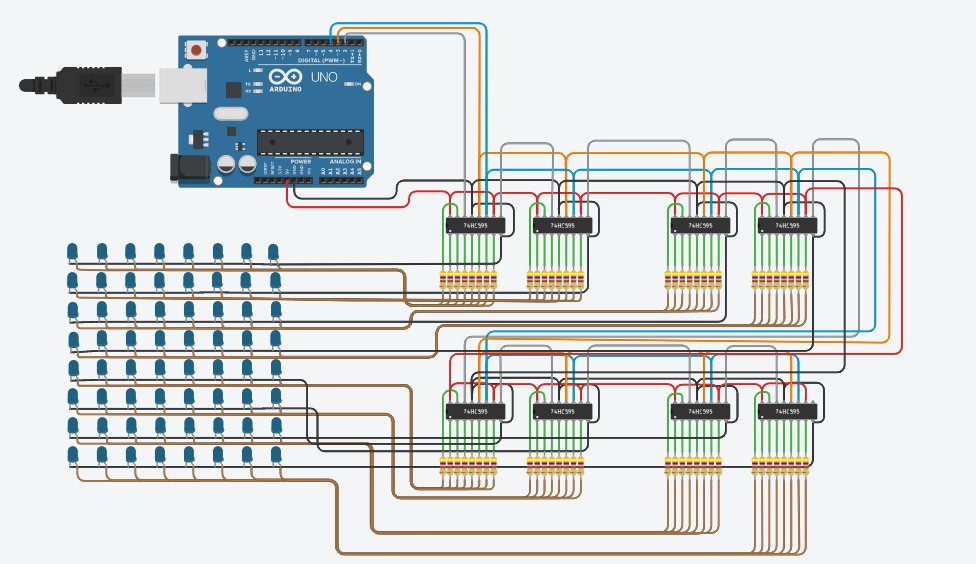
\includegraphics[width=10cm]{Tinkercar.jpeg}
\centering
\caption{Tinkercar}
\label{fig:gestion}
\end{figure}


 
 \vspace{1cm}
 
  *Pines integrado 1 y 2*

\vspace{1cm}


\vspace{8cm}
\section{Conclusión} \label{conclulsion}




\vspace{1cm}


\end{document}
